% Generated by figures/gen_phase4_paper_assets.py
\begin{figure*}[t]
    \centering
    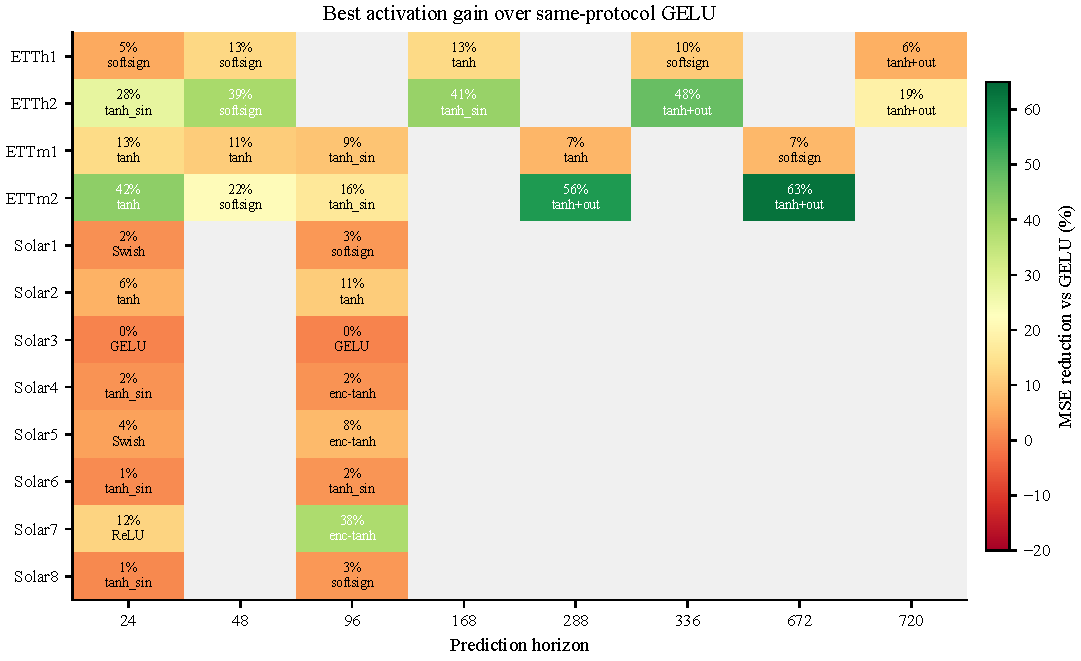
\includegraphics[width=\textwidth]{figures/fig_phase4_best_gain_heatmap.pdf}
    \caption{Best activation gain over the same-protocol GELU row in each completed dataset-horizon cell. The full grid covers 36 dataset-horizon cells, nine activation configurations, and three seeds. Most cells prefer a non-GELU activation, but Solar3 remains GELU-best at both horizons.}
    \label{fig:phase4_best_gain_heatmap}
\end{figure*}

\begin{figure}[t]
    \centering
    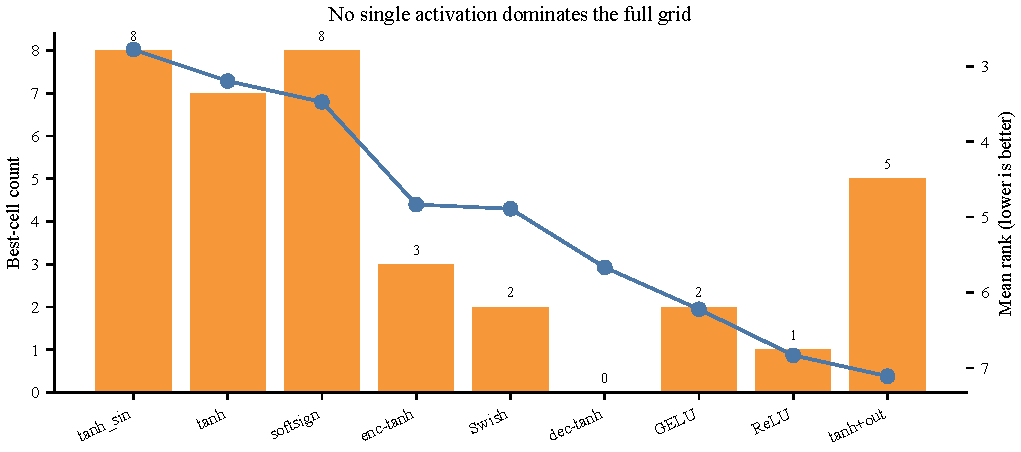
\includegraphics[width=\linewidth]{figures/fig_phase4_static_ranking.pdf}
    \caption{Static activation ranking across the full Phase-4 grid. Bounded and tanh-family activations rank best on average, but the best-cell counts are spread across several configurations, arguing against a universal replacement activation.}
    \label{fig:phase4_static_ranking}
\end{figure}
